\documentclass{jarticle}

\usepackage[dvipdfmx]{graphicx}
\usepackage{float}

\title{重力加速度の測定}
\author{2511198 肥田幸久}
\date{2025年5月4日}

\begin{document}
\maketitle

\section{実験の目的}

本実験では, ボルダの振り子を用いて精密に測定した振り子の周期から, 電気通信大学における重力加速度の値を4桁の精度で測定する.


\section{実験の原理}


\subsection{重力加速度}

地球を球形と仮定し, 質量を$M$, 半径を$R$, 万有引力定数を$G$とすると, 地球上の質量$m$の物体に働く重力の大きさ$mg$は
\begin{equation}
  mg=GMm/R^2
\end{equation}
と表され, 重力加速度$g$は
\begin{equation}
  g=GM/R^2
\end{equation}
と表される. また, この式に
\begin{itemize}
  \item $G=6.674\times10^{-11}\,\mathrm{N\cdot m^2/kg^2}$
  \item $M=5.972\times10^{24}\,\mathrm{kg}$,
  \item $R=6.378\times10^6\,\mathrm{m}$,
\end{itemize}
を代入して計算すると[1]
\begin{equation}
  g=9.798\,\mathrm{m/s^2}
\end{equation}
を得る.
したがって重力加速度のおおよその大きさは$g=9.8\,\mathrm{m/s^2}$である.


\subsection{振り子の周期と重力加速度}

単振り子の振動の周期は重力加速度と関係している. 振り子の長さを$h$とすると, その周期$T$は
\begin{equation}
  \label{equ:T-from-G}
  T=2\pi\sqrt{\frac{h}{g}}
\end{equation}
で表される.
この式は, 振り子のおもりと振動の振幅が小さい場合の近似式であるが, この式を使えば振り子の周期$T$を測ることで重力加速度$g$は
\begin{equation}
  \label{equ:G-from-T-1}
  g=\frac{4\pi^2h}{T^2}
\end{equation}
と求めることができる.

しかし, この式で重力加速度の値を4桁の精度で求めることは難しい.
仮に振り子の長さを$h=1\,\mathrm{m}$とすると, 周期は約2秒となる.
式(\ref{equ:G-from-T-1})中の$h$を4桁の精度で求めるためには, 振り子の長さを不確かさ$1\,\mathrm{mm}$以内で測る必要があるが, これは容易である.
それに対して, 式(\ref{equ:G-from-T-1})中の$T^2$を4桁の精度で求めるためには, 30周期をストップウォッチで測る場合には時間測定の不確かさを0.06秒以内, 60周期の場合にも0.12秒以内にする必要があるが, これは容易ではない.

この例からわかるように, $g$を精密に測るためには周期をもっと精度よく測定する必要がある.


\subsection{より精密な周期測定}

約2秒の周期で振動する振り子に, $T_0=2\,\mathrm{s}$毎に光パルスを照射すると, 暗い視野の中で振り子の吊り線が2秒毎に白く輝いて見える.
もし振り子の周期$T$が$T_0=2\,\mathrm{s}$とわずかに異なっている場合, 2秒毎に光パルスに照らされる金属線の位置は少しずつずれていく.
そしてこの白く輝く金属線の動きは, 周期の長い単振動である.
この長い周期$\tau$から, 振り子の周期$T$は次の式から求めることができる.
\begin{equation}
  \frac{1}{T_0}-\frac{1}{T}=\frac{\pm1}{\tau}
\end{equation}
\begin{equation}
  T=T_0\pm\frac{T_0^2}{\tau\mp T_0}
\end{equation}
複号は振り子の周期$T$が$T_0$よりも長いときは上を, 短いときは下をとる.
今回の実験では$T$が$T_*0$より長いため以下の式になる.
\begin{equation}
  \label{eq:T-from-tau}
  T=T_0+\frac{T_0^2}{\tau-T_0}
\end{equation}


\subsection{より精密な重力加速度の計算}

前述したとおり, 式(\ref{equ:T-from-G})は次の仮定のもとに導かれたものである.
\begin{itemize}
  \item おもりの大きさが無視できる
  \item 振動の振幅が十分に小さい
\end{itemize}
ここではおもりの大きさの影響と, 振り子の振幅の影響を考慮する.

おもりを半径$r$の球体とし, 振り子の最大振れ角を$\theta$とすると, 次の式でより近似した周期を表せる.
\begin{equation}
  T=2\pi\sqrt{\frac{h}{g}\left(1+\frac{2r^2}{5h^2}\right)}\left(1+\frac{\theta^2}{16}\right)
\end{equation}
これより$g$は
\begin{equation}
  \label{eq:G-from-T-2}
  g=\frac{4\pi^2h}{T^2}\left(1+\frac{2r^2}{5h^2}\right)\left(1+\frac{\theta^2}{8}+\frac{\theta^4}{256}\right)
\end{equation}
と求めることができる.


\section{実験方法}

この実験では以下のような装置を用いて測定を行った.
直径$d$の鋼球を太さ$0.2\,\mathrm{mm}$のピアノ線で吊るし, ピアノ線の上部をナイフエッジの付いた金具に固定する.
ナイフエッジを水平な金属板の上に乗せて鋼球を振動させる.
この装置は, ボルダの振り子と呼ばれている.

\begin{figure}[H]
  \begin{center}
  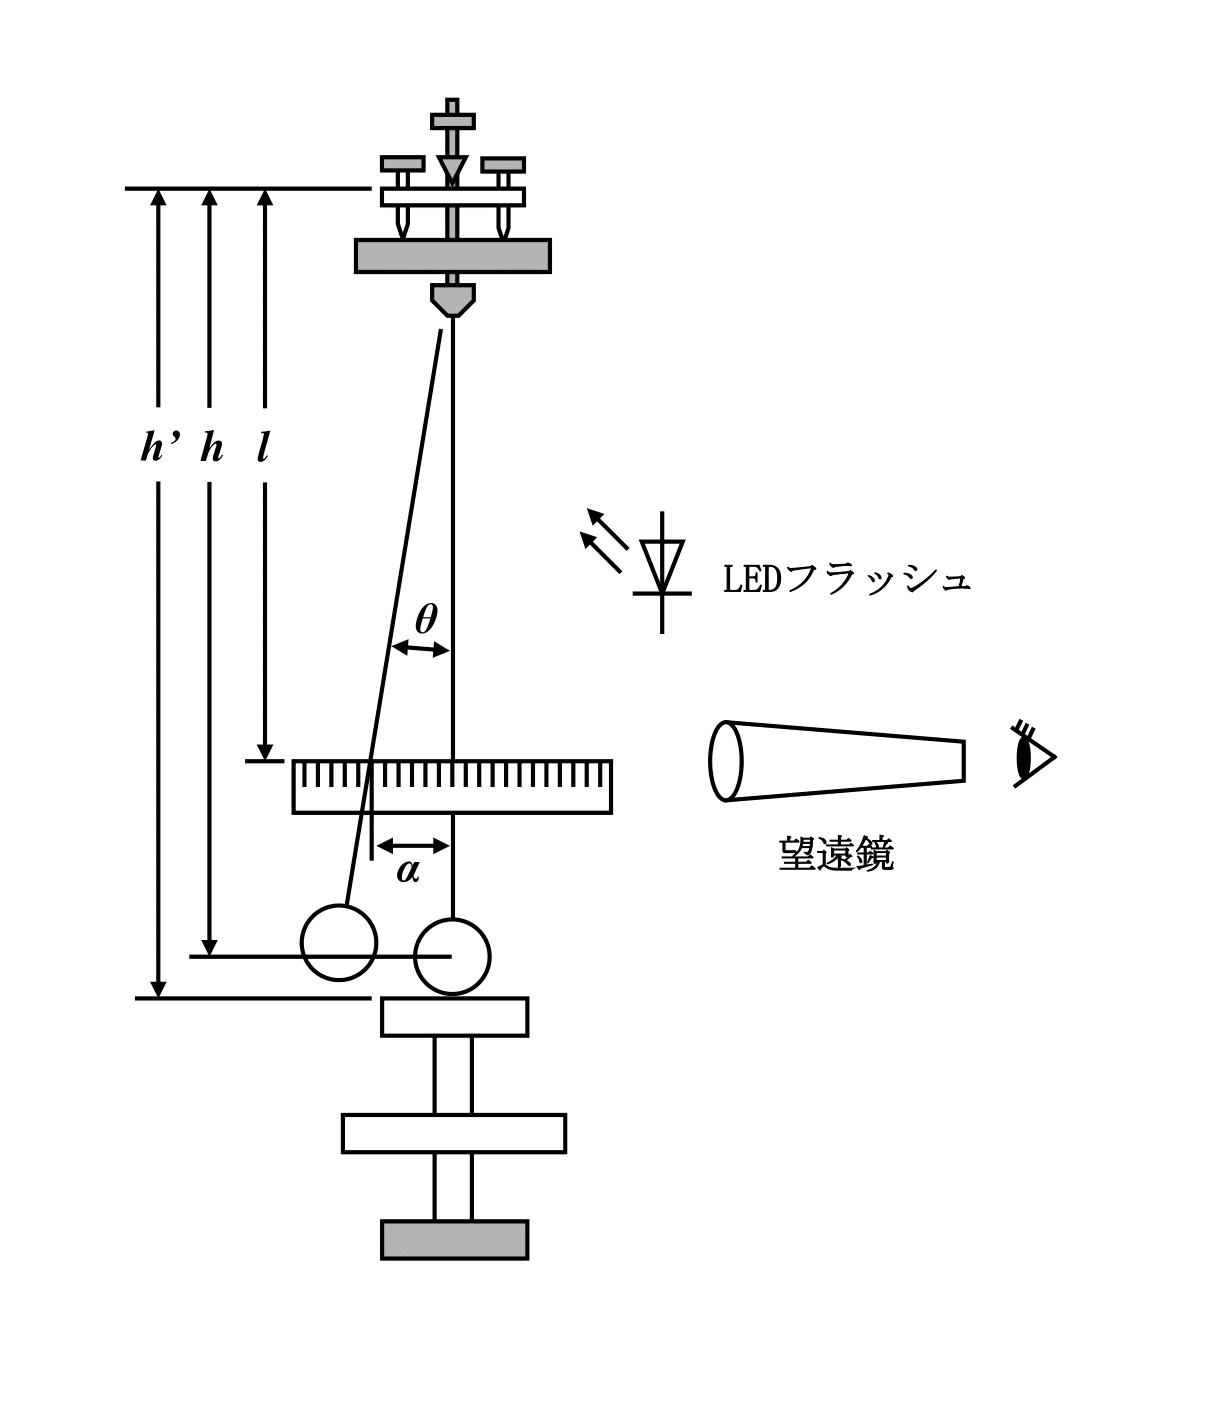
\includegraphics[width=60mm]{experimental_method_picture.png}
  \caption{振り子の実験装置}
  \end{center}
\end{figure}

正確に2秒ごとに発光するLEDフラッシュランプの光パルス(時間間隔の不確かさは$1$\textmu s以内, 発光時間は約$10$\textmu s)で振り子を照射する.
光パルスに照らされて光るピアノ線を望遠鏡で観察し, 白く光るピアノ線が左右に往復する周期$\tau$を測定する.


\section{実験結果}

今回の実験では, 振り子の長さを4通り変えて実験を行った.
以下に, 今回の実験を通して変化しない初期値(表\ref{tb:initial-value-1}), それぞれの測定ごとに変化する初期値(表\ref{tb:initial-value-2}), および光るピアノ線の周期の測定結果(表\ref{tb:measure-result})を示す.

\begin{table}[h]
  \centering
  \caption{実験の初期値}
  \begin{tabular}{ccc}
    \hline
    & $d/\mathrm{mm}$ & $l/\mathrm{mm}$\\
    \hline
    & $25.5$ & $886.5$ \\
    & $25.4$ & $880.5$ \\
    & $25.5$ & $881.5$ \\
    \hline
    平均 & 25.5 & 882.8 \\
    \hline
  \end{tabular}
  \label{tb:initial-value-1}
\end{table}

\begin{table}[h]
  \centering
  \caption{測定ごとの初期値}
  \begin{tabular}{cc|cc}
    \hline
    & $h/\mathrm{mm}$ & & $\alpha/\mathrm{mm}$ \\
    \hline
    $h_1$ & 1043.1 & $\alpha_1$ & 2.05 \\
    $h_2$ & 1037.1 & $\alpha_2$ & 13.3 \\
    $h_3$ & 1026.7 & $\alpha_3$ & 19.4 \\
    $h_4$ & 1016.5 & $\alpha_4$ & 18.0 \\
    \hline
  \end{tabular}
  \label{tb:initial-value-2}
\end{table}

\begin{table}[h]
  \centering
  \caption{光るピアノ線の周期の測定結果}
  \begin{tabular}{ccccc}
    \hline
     & \multicolumn{3}{c}{周期\,$\tau/\mathrm{s}$} \\
    回数 & $h_1,\alpha_1$ & $h_2,\alpha_2$ & $h_3,\alpha_3$ & $h_4,\alpha_4$ \\
    \hline
    1 & 84.02 & 92.60 & 122.20 & 244.17 \\
    2 & 83.86 & 91.80 & 124.01 & 241.98 \\
    3 & 84.32 & 92.81 & 121.96 & 243.89 \\
    \hline
    平均 & 84.07 & 92.40 & 122.72 & 243.35 \\
    \hline
  \end{tabular}
  \label{tb:measure-result}
\end{table}

表\ref{tb:measure-result}の平均値より, 式(\ref{eq:T-from-tau})を用いて振り子の周期$T$を求め, 次にここで求めた周期$T$より, 式(\ref{eq:G-from-T-2})を用いて重力加速度$g$を求める. これらの計算結果とその平均値, すなわち実験結果を以下の表\ref{tb:experiment-result}に示す. 

\begin{table}[H]
  \centering
  \caption{ボルダの振り子による重力加速度の測定結果}
  \begin{tabular}{ccc}
    \hline
    & 周期\,$T/\mathrm{s}$ & 重力加速度\,$g/\mathrm{ms^{-2}}$\\
    \hline
    1 & 2.0487 & 9.8116 \\
    2 & 2.0442 & 9.7983 \\
    3 & 2.0331 & 9.8067 \\
    4 & 2.0166 & 9.8694 \\
    \hline
    平均 & & 9.8215 \\
    \hline
  \end{tabular}
  \label{tb:experiment-result}
\end{table}

\begin{table}[h]
  \centering
  \caption{ボルダの振り子による重力加速度の測定結果}
  \begin{tabular}{ccc}
    \hline
    & 測定値 & 文献値 \\
    \hline
    $g/\mathrm{ms^{-2}}$ & 9.8215 & 9.7969 \\
    \hline
  \end{tabular}
\end{table}

よって本実験では, ボルダの振り子を用いて, 電気通信大学における重力加速度の値を$9.8215\,\mathrm{m/s^2}$と測定した.


\section{考察}


\subsection{実験結果の分析}

本実験では, 振り子の長さを4通り変えて実験を行ったが, 求めた重力加速度の4通りの値のなかで4つ目の値のみが他の値と大きく異なっている.
本実験では重力加速度$g$に対する不確かさ$\Delta g$を計算する際に必要な数値を実験中に求めなかったため, 4つ目の値を平均処理から除外できない.
そこで, 以下のテキストに記載されている値および式を用いて重力加速度の不確かさ$\Delta g$を求める. ただし, $\Delta h'$に関しては実測値のばらつきから, $\Delta h'=0.2\,\mathrm{mm}$とする.

\begin{itemize}
  \item $\Delta\tau=1\,\mathrm{s}$
  \item $\Delta h'=0.2\,\mathrm{mm}$
  \item $\Delta d=0.05\,\mathrm{mm}$
  \item $g=10\,\mathrm{m/s^2}$
  \item $h=1\,\mathrm{m}$
  \item $T=2\,\mathrm{s}$
\end{itemize}

\begin{equation}
  \frac{\Delta g}{g}=\sqrt{\left(\frac{\Delta h}{h}\right)^2+\left(\frac{2\Delta T}{T}\right)^2}
\end{equation}

\begin{equation}
  \bar{g}=\frac{
    \frac{g_1}{(\Delta g_1)^2} + \frac{g_2}{(\Delta g_2)^2}+\cdots+\frac{g_n}{(\Delta g_n)^2}
  }{
    \frac{1}{(\Delta g_1)^2} + \frac{2}{(\Delta g_2)^2}+\cdots+\frac{1}{(\Delta g_n)^2}
  }
\end{equation}

\begin{table}[H]
  \centering
  \caption{重力加速度の不確かさ}
  \begin{tabular}{ccc}
    \hline
    & $g/\mathrm{ms^{-2}}$ & $\Delta g/\mathrm{ms^{-2}}$ \\
    \hline
    1 & 9.8116 & $\pm 0.0060$ \\
    2 & 9.7983 & $\pm 0.0051$ \\
    3 & 9.8067 & $\pm 0.0033$ \\
    4 & 9.8694 & $\pm 0.0021$ \\
    \hline
  \end{tabular}
\end{table}

これより,4つ目の値では重大な測定ミスがあったと思われる. そのため, 4つ目の値を除外し平均処理を行うと, $\bar{g}=9.8055\,\mathrm{m/s^2}$と求められる. これは過去電気通信大学にて原子干渉計を用いた高度な重力加速度計による$g=9.7969\,\mathrm{m/s^2}$に近い値である.[2]


\subsection{課題(1)}

重力加速度は, 緯度が高いほど大きくなる.
そのため日本国内において重力加速度の値が最も大きな所は日本最北端の択捉島であり,もっとも小さな所は日本最南端の沖ノ鳥島である.


\subsection{課題(3)}

本実験における吊り線の質量$m$は, ピアノ線の密度を$7.85\,\mathrm{g/cm^3}$とすると, [3]$m=0.2466\,\mathrm{g}$であり, これは鋼球の質量に対して極わずかであるため, 厳密には考慮するべきだが今回の実験においては考慮する必要はない.


\subsection{課題(4)}


\subsubsection{\textcircled{\scriptsize 1}}

$g=9.5106\times10^{-6}\,\mathrm{m/s^2}$

この数値は, 今回の実験の精度をはるかに下回っている.


\subsubsection{\textcircled{\scriptsize 2}}

\begin{table}[H]
  \centering
  \caption{高層ビルにおける重力加速度の差}
  \begin{tabular}{cc}
    \hline
    & $g/\mathrm{ms^{-2}}$ \\
    \hline
    1階 & 9.798 \\
    最上階($l=300\,\mathrm{m}$) & 9.797 \\
    \hline
    差 & 0.001 \\
    \hline
  \end{tabular}
\end{table}

標高を$300\,\mathrm{m}$の変化が無い限り, 標高は今回の実験の精度には影響を及ぼさない.


\subsubsection{\textcircled{\scriptsize 3}}

東に速度$10\,\mathrm{m/s}$で運動している乗り物内での重力加速度の減少量は, \\
$\Delta g=1.114\times10^{-3}\,\mathrm{m/s^2}$である. これは今回の実験の精度に確実に影響を及ぼす.


\section{参考文献}

[1] 東京都市大学, ボルダの振り子による重力加速度の測定

[2] 小田悠介, 原子干渉計を用いた高精度な重力加速度計の開発, 電気通信大学大学院 電気通信学研究科 量子・物質工学専攻 中川研究室

[3]日本ミニチュアロープ(株), 素材と特性

  

\end{document}